\section{Valuation}
\label{sec:valuation}

\subsection{The coupled moment system}
\label{sec:moments}

Pricing requires $\mu_X(t)$ for the centring in \eqref{eq:centering} and the
conditional distribution of $X_T$ for the payoff. Both follow from a system of
regime-partitioned moments. Define
\begin{equation}
  p_i(t)=\Q\!\left(S_t=i\right),\qquad
  u_i(t)=\E^{\Q}\!\left[X_t\mathbf{1}_{\{S_t=i\}}\right],\qquad
  w_i(t)=\E^{\Q}\!\left[X_t^{2}\mathbf{1}_{\{S_t=i\}}\right],
\end{equation}
for $i\in\{0,1\}$. Applying the Kolmogorov forward equation for the chain and
Itô's lemma to \eqref{eq:ou} on each regime-restricted expectation yields a
closed six-dimensional linear system. The property that matters for what follows
is its recursive structure: $p$ evolves autonomously, $u$ depends on $p$, and $w$
depends on both, so the system is linear and no closure approximation is
required.
\begin{equation}
\begin{aligned}
  \dot p_0 &= -q_{01}p_0 + q_{10}p_1,\\[2pt]
  \dot p_1 &= \phantom{-}q_{01}p_0 - q_{10}p_1,\\[4pt]
  \dot u_0 &= \kappa\left(m_0 p_0 - u_0\right)
              + a_0 p_0 - q_{01}u_0 + q_{10}u_1,\\[2pt]
  \dot u_1 &= \kappa\left(m_1 p_1 - u_1\right)
              + a_1 p_1 + q_{01}u_0 - q_{10}u_1,\\[4pt]
  \dot w_0 &= 2\kappa\left(m_0 u_0 - w_0\right)
              + 2a_0 u_0 + \left(\sigma^X_0\right)^{2}p_0
              - q_{01}w_0 + q_{10}w_1,\\[2pt]
  \dot w_1 &= 2\kappa\left(m_1 u_1 - w_1\right)
              + 2a_1 u_1 + \left(\sigma^X_1\right)^{2}p_1
              + q_{01}w_0 - q_{10}w_1,
\end{aligned}
\label{eq:momentsys}
\end{equation}
initialised at $p_i(0)=\pi_i$, $u_i(0)=x_0\pi_i$, $w_i(0)=x_0^{2}\pi_i$, where
$\pi$ is the filtered regime distribution at the valuation hour and $x_0=0$.
The terms in $a_i$ carry the risk-neutral drift perturbation of
Section~\ref{sec:q1} and are zero in the baseline.

The unconditional moments follow by summation,
\begin{equation}
  \mu_X(t) = u_0(t)+u_1(t),
  \qquad
  \operatorname{Var}^{\Q}\!\left[X_t\right]
    = w_0(t)+w_1(t) - \mu_X(t)^{2},
\end{equation}
which establishes the representation used in the proof of
Proposition~\ref{prop:centering}.

One numerical point is worth stating here because it was a failure mode in
development. The coefficients $q_{01},q_{10}$ and $\sigma^X_i$ vary along the
covariate path, so \eqref{eq:momentsys} is non-autonomous and cannot be advanced
by matrix exponentials on a coarse grid; on hourly steps the second-moment
trajectory was visibly unstable. Appendix~\ref{app:numerics} gives the
integration scheme adopted in response.

\subsection{Pricing equation}

Conditional on the regime, the value function $V_i(x,t)$ for regime $i$ solves
the coupled system
\begin{equation}
  \frac{\partial V_i}{\partial t}
  + \left[\kappa\left(m_i-x\right)+a_i\right]\frac{\partial V_i}{\partial x}
  + \tfrac12\left(\sigma^X_i(t)\right)^{2}\frac{\partial^{2}V_i}{\partial x^{2}}
  - rV_i
  + q_{ij}(t)\left(V_j - V_i\right) = 0,
  \qquad j\neq i,
  \label{eq:pde}
\end{equation}
with terminal condition $V_i(x,T) = \left(F(T)+x-\mu_X(T)-K\right)^{+}$ for a
call. The coupling term $q_{ij}(V_j-V_i)$ is the regime-switching contribution
familiar from \citet{BuffingtonElliott2002} and \citet{JobertRogers2006}; the
numerical treatment follows the finite-difference approach of
\citet{BoyleDraviam2007} and \citet{Huang2011}. We discretise $x$ on a uniform
grid of $1{,}201$ nodes spanning a domain wide enough that the terminal density
is numerically negligible at the boundaries, and we report the option value as
the $\pi$-weighted mixture $V_0(0,0)\pi_0 + V_1(0,0)\pi_1$.

The drift term in \eqref{eq:pde} and the $a_i$ terms in \eqref{eq:momentsys}
must be populated from the same parameter field. This is a genuine hazard
rather than a housekeeping remark: adding a perturbation to the moment system
alone, or to the pricing equation alone, breaks Proposition~\ref{prop:centering}
silently, producing prices that remain plausible while no longer being anchored
to the forward. We guard against it with a regression test that asserts
$\max_t\lvert\E^{\Q}[P_t]-F(t)\rvert < 10^{-8}$ \TRY{} across asymmetric,
mixed-sign perturbation pairs, and which fails if the two code paths are ever
allowed to diverge.

\subsection{Independent verification}

Two checks discipline the numerics. First, put--call parity,
$C-P = e^{-rT}\left(F(T)-K\right)$, holds by no-arbitrage independently of the
model and provides an internal consistency test. Across the full
strike--maturity grid of Section~\ref{sec:surface} the maximum absolute parity
error is $1.0\times10^{-6}$ \TRY, which is solver precision.

Second, \eqref{eq:ou} is simulated directly with an exact conditional
Ornstein--Uhlenbeck step on the sampled regime path, $4\times10^{4}$ paths at a
$0.05$-hour time step, and compared against the finite-difference solution across
strikes (Figure~\ref{fig:pdemc}). The two routes share only the parameter file:
one integrates a deterministic moment system and solves a boundary-value problem,
the other samples trajectories. They agree to within roughly $1\%$ near the money.
The residual discrepancy is systematic rather than random, with Monte Carlo below
the finite-difference value at every strike and the gap widening from $0.6\%$ at
$K=2{,}000$ to $3.1\%$ at $K=4{,}000$. This is the signature of time
discretisation in the sampled regime path: switching events occurring within a
step are missed, which slightly understates mixing into the high-volatility state
and therefore the deep out-of-the-money tail on which far strikes depend. Since
the effect is concentrated where option values are smallest in absolute terms, it
does not affect the conclusions drawn here, but it does mean the Monte Carlo
figures should be read as a consistency check rather than as an independent
valuation.

\begin{figure}[htbp]
\centering
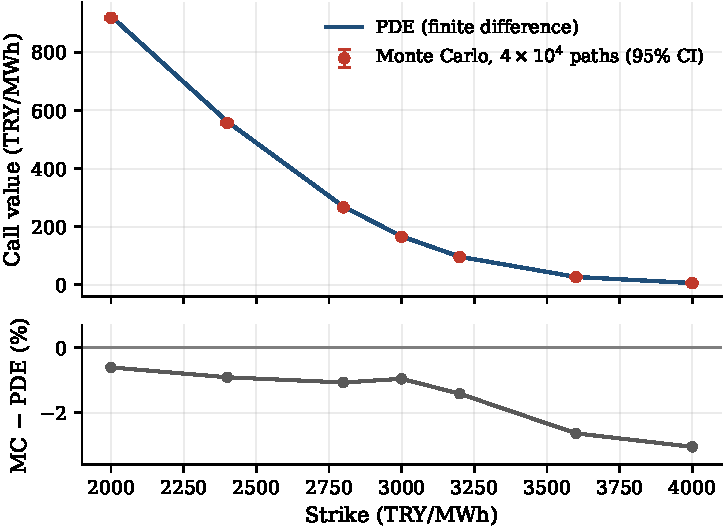
\includegraphics[width=\textwidth]{figures/pde_mc.pdf}
\caption{Finite-difference against Monte Carlo call values at $72$ hours, with
the relative difference below.}
\label{fig:pdemc}
\end{figure}

Agreement of this kind is informative about implementation correctness. It says
nothing about whether the parameters describe the market.

\subsection{The risk-neutral drift channel}
\label{sec:q1}

The regime and volatility parameters of Section~\ref{sec:residual} are
historical estimates under $\PP$. Using them unchanged for valuation asserts
that the market prices neither regime nor volatility risk. Since the monthly
strip cannot identify either premium, we do not attempt to estimate them.
Instead we implement the change of measure explicitly so that the assumption
becomes visible and its consequences measurable.

Following the structure in \citet{Janczura2014}, we admit a regime-dependent
drift perturbation, replacing \eqref{eq:ou} by
\begin{equation}
  \dif X_t = \left[\kappa\left(m_{S_t}-X_t\right) + a_{S_t}\right]\dif t
             + \sigma^X_{S_t}(t)\,\dif W^{\Q}_t,
  \label{eq:q1}
\end{equation}
with $a=(a_0,a_1)$ expressed in \TRY{} per hour. Setting $a=(0,0)$ recovers the
physical-measure baseline exactly, bit for bit, so every result in this paper
that does not explicitly vary $a$ is a zero-premium result and is labelled as
such.

The perturbation enters \eqref{eq:momentsys} through $a_ip_i$ in the first moment
and $2a_iu_i$ in the second, so the effect on the variance, and hence on option
value, is second order in $a$. Appendix~\ref{app:moments} derives the order and
reports the numerical check, a log-log slope of $2.0000$ across
$a_1\in\{-0.5,\dots,-20\}$. At magnitudes plausible for a drift premium the
resulting price change falls below the solver's resolution. The implication is
specific: within this specification a \emph{drift}-type premium is nearly
unidentifiable from option values even if one were observed, because its channel
is quadratically suppressed. A premium shifting transition intensities rather
than drift would not be suppressed in the same way, and that extension is left
open.
